\section{Analyse Paramétrique}

On observe sur la figure~\ref{fig:analyseParam} qu'il y a seulement l'eau 
qui varie avec la température.
Les autres composés ne varient donc qu'avec la quantité de \ce{NH3} à produire.

\begin{figure}[h!]
	\begin{center}
		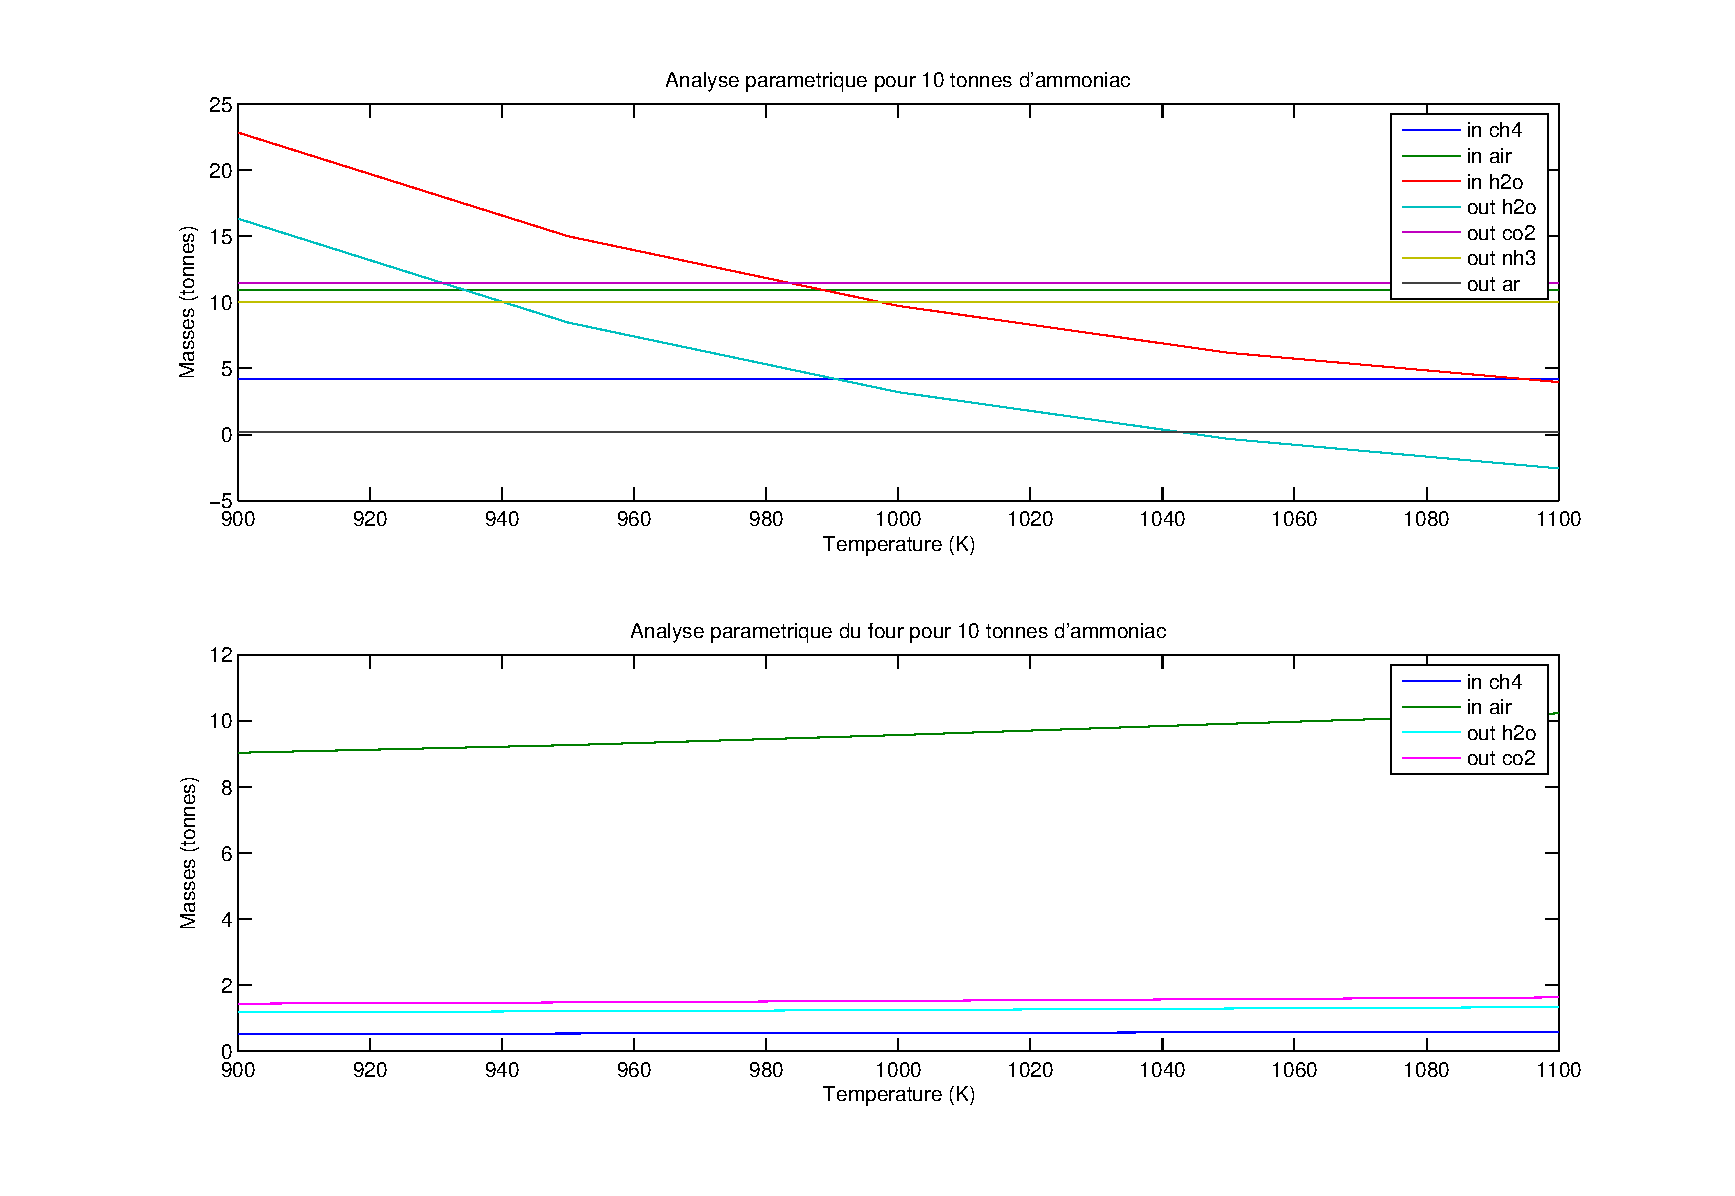
\includegraphics[scale=0.5]{../tache1/img/analyseParam.eps}
	\end{center}
	\caption{Analyse paramétrique pour $10$ tonnes de \ce{NH3}
		le graphe supérieur représente les flux de l'ensemble du 
		procédé, depuis le reformeur primaire jusqu'au réacteur de synthèse.}
	\label{fig:analyseParam}
\end{figure}


